% IT Ethics Lecture 4: Intellectual Property
% Brendan Shea, PhD
% Rochester Community and Technical College

\documentclass[aspectratio=169]{beamer}

% Theme and colors
\usetheme{Madrid}
\usecolortheme{whale}
\setbeamertemplate{navigation symbols}{}
\setbeamertemplate{footline}[frame number]

% Packages
\usepackage[utf8]{inputenc}
\usepackage[T1]{fontenc}
\usepackage{graphicx}
\usepackage{booktabs}
\usepackage{array}
\usepackage{multirow}
\usepackage{hyperref}
\usepackage{csquotes}

% TikZ and libraries
\usepackage{tikz}
\usetikzlibrary{shapes.geometric, arrows.meta, positioning, calc, backgrounds, fit, decorations.pathreplacing, shadows}

% Custom colors
\definecolor{primaryblue}{RGB}{0,74,124}
\definecolor{accentorange}{RGB}{230,126,34}
\definecolor{lightgray}{RGB}{245,245,245}
\definecolor{darktext}{RGB}{44,62,80}

% Customize blocks
\setbeamercolor{block title}{bg=primaryblue, fg=white}
\setbeamercolor{block body}{bg=lightgray, fg=darktext}
\setbeamercolor{block title example}{bg=green!60!black, fg=white}
\setbeamercolor{block body example}{bg=green!10, fg=darktext}
\setbeamercolor{block title alerted}{bg=red!70!black, fg=white}
\setbeamercolor{block body alerted}{bg=red!10, fg=darktext}

% Title information
\title[IT Ethics: Lecture 4]{Intellectual Property}
\subtitle{Ideas, Ownership, and the Digital Age}
\author{Brendan Shea, PhD}
\institute[RCTC]{Rochester Community and Technical College}
\date{}

\begin{document}

%------------------------------------------------------
% SLIDE 1: Title Slide
%------------------------------------------------------
\begin{frame}
\titlepage
\end{frame}

%------------------------------------------------------
% SLIDE 2: What Is Intellectual Property?
%------------------------------------------------------
\begin{frame}{What Is Intellectual Property?}
    \begin{itemize}
        \item \textbf{Intellectual property (IP)} refers to legal rights granted over creations of the mind, including inventions, artistic works, designs, and brand names.
        \item Unlike physical property such as land or cars, intellectual property is \textbf{non-rivalrous}---my using an idea doesn't prevent you from using the same idea simultaneously.
        \item IP law creates artificial scarcity by granting creators temporary exclusive rights, allowing them to control who uses their creations and to profit from that control.
        \item The major forms of IP include \textbf{patents} (inventions), \textbf{copyrights} (creative works), \textbf{trademarks} (brand identifiers), and \textbf{trade secrets} (confidential business information).
    \end{itemize}
    
    \vspace{0.3em}
    
    \begin{block}{Physical vs. Intellectual Property}
        If I take your bicycle, you no longer have it. But if I copy your song, you still have it too---we both do. This fundamental difference makes IP philosophically puzzling: why grant exclusive rights over something that can be infinitely shared?
    \end{block}
\end{frame}

%------------------------------------------------------
% SLIDE 3: Why Does Intellectual Property Matter?
%------------------------------------------------------
\begin{frame}{Why Does Intellectual Property Matter?}
    \begin{itemize}
        \item IP-intensive industries---including software, pharmaceuticals, entertainment, and manufacturing---account for trillions of dollars in economic activity and millions of jobs worldwide.
        \item Intellectual property shapes everyday life: the music you stream, the medicines you take, the apps on your phone, and the brands you recognize are all governed by IP law.
        \item IP rules determine what you can legally create, share, remix, and repair---affecting everything from posting memes to fixing your own tractor.
        \item Debates over IP have intensified in the digital age, as copying and sharing have become nearly costless while enforcement has become increasingly difficult.
    \end{itemize}
    
    \vspace{0.3em}
    
    \begin{table}[h]
        \centering
        \footnotesize
        \begin{tabular}{lrr}
            \toprule
            \textbf{Industry} & \textbf{U.S. GDP Contribution} & \textbf{Jobs (millions)} \\
            \midrule
            Software \& IT & \$1.8 trillion & 3.4 \\
            Pharmaceuticals & \$650 billion & 0.9 \\
            Film \& Music & \$470 billion & 2.5 \\
            Publishing & \$280 billion & 1.1 \\
            \bottomrule
        \end{tabular}
    \end{table}
\end{frame}

%------------------------------------------------------
% SLIDE 4: The Central Tension
%------------------------------------------------------
\begin{frame}{The Central Tension}
    \begin{itemize}
        \item \textbf{Creators} want recognition, control, and financial reward for their work---without protection, others could simply copy and profit from their efforts.
        \item \textbf{Society} benefits when ideas spread freely, allowing others to build on existing knowledge, create new works, and access information without barriers.
        \item Every intellectual property system must balance these competing interests, and different societies at different times have struck very different balances.
        \item Finding the right balance is genuinely difficult: too little protection may discourage creation, while too much protection may lock away knowledge and stifle innovation.
        \end{itemize}
        
        \vspace{0.5em}
        
        \centering
        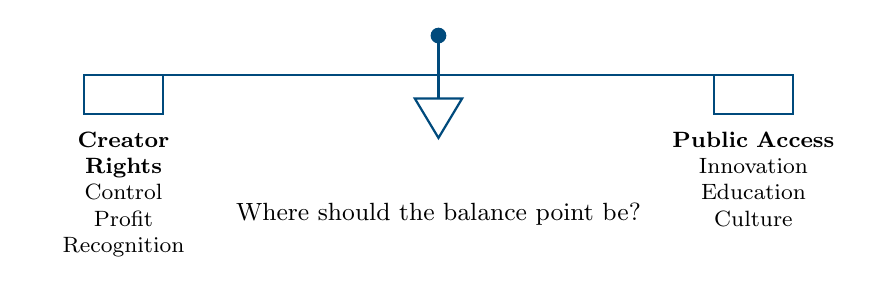
\begin{tikzpicture}[scale=1.0]
        % Balance beam
        \draw[thick, primaryblue] (-4,0) -- (4,0);
        \draw[thick, primaryblue] (0,-0.3) -- (0,0.5);
        \fill[primaryblue] (0,0.5) circle (0.1);
        
        % Left pan (Creator Rights)
        \draw[thick, primaryblue] (-3.5,-0.5) -- (-3.5,0) -- (-4.5,0) -- (-4.5,-0.5) -- cycle;
        \node[below, font=\footnotesize, text width=2.2cm, align=center] at (-4,-0.6) {\textbf{Creator Rights}\\Control\\Profit\\Recognition};
        
        % Right pan (Public Access)
        \draw[thick, primaryblue] (3.5,-0.5) -- (3.5,0) -- (4.5,0) -- (4.5,-0.5) -- cycle;
        \node[below, font=\footnotesize, text width=2.2cm, align=center] at (4,-0.6) {\textbf{Public Access}\\Innovation\\Education\\Culture};
        
        % Fulcrum
        \draw[thick, primaryblue] (-0.3,-0.3) -- (0.3,-0.3) -- (0,-0.8) -- cycle;
        
        % Question
        \node[below, font=\small] at (0,-1.5) {Where should the balance point be?};
        \end{tikzpicture}
\end{frame}

%------------------------------------------------------
% SLIDE 5: A Brief History of Intellectual Property
%------------------------------------------------------
\begin{frame}{A Brief History of Intellectual Property}
    \begin{itemize}
        \small
        \item The first known patent law was enacted in \textbf{Venice in 1474}, granting glassblowers exclusive rights to their techniques for ten years to encourage innovation and prevent trade secrets from leaving the city.
        \item The \textbf{Statute of Anne} (England, 1710) was the first modern copyright law, granting authors---not publishers---rights to their works for a limited 14-year term.
        \item The U.S. Constitution (1787) explicitly empowers Congress to grant IP rights ``to promote the Progress of Science and useful Arts''---notably framing IP as a \textit{means} to public benefit, not an end in itself.
        \item IP protections have expanded dramatically over time: copyright terms have grown from 14 years to life plus 70 years, and patent coverage has extended to software, business methods, and genes.
    \end{itemize}
    
    \vspace{0.3em}
    
    \begin{table}[h]
        \centering
        \footnotesize
        \begin{tabular}{lll}
            \toprule
            \textbf{Year} & \textbf{Development} & \textbf{Significance} \\
            \midrule
            1474 & Venetian Patent Statute & First formal patent system \\
            1710 & Statute of Anne & First copyright law; author's rights \\
            1787 & U.S. Constitution & IP as tool for public progress \\
            1998 & DMCA / Sonny Bono Act & Digital controls; extended terms \\
            \bottomrule
        \end{tabular}
    \end{table}
\end{frame}

%------------------------------------------------------
% SLIDE 6: Utilitarian Justifications for IP
%------------------------------------------------------
\begin{frame}{Utilitarian Justifications for IP}
    \begin{itemize}
        \item The \textbf{utilitarian} approach, associated with philosophers like Bentham and Mill, holds that IP is justified only if it produces the greatest good for the greatest number.
        \item The core argument: without legal protection, creators cannot profit from their work because competitors will simply copy it, so fewer people will invest time and resources in creating new things.
        \item IP creates a \textbf{temporary monopoly} as an incentive---the creator gets exclusive rights for a limited time, after which the work enters the public domain for everyone to use.
        \item On this view, IP is a necessary evil: monopolies are generally bad, but the innovation they encourage outweighs the costs of restricted access.
    \end{itemize}
    
    \vspace{0.3em}
    
    \begin{quote}
        \footnotesize
        ``Considering the exclusive right to invention as given not of natural right, but for the benefit of society, I know well the difficulty of drawing a line between the things which are worth to the public the embarrassment of an exclusive patent, and those which are not.'' \\ \hfill ---Thomas Jefferson
    \end{quote}
\end{frame}

%------------------------------------------------------
% SLIDE 7: Utilitarian Trade-offs: Incentives vs. Access
%------------------------------------------------------
\begin{frame}{Utilitarian Trade-offs: Incentives vs. Access}
    \begin{itemize}
        \item \textbf{Too little protection}: Creators can't recoup investments, leading to less innovation---why spend years developing a drug if competitors can copy it immediately?
        \item \textbf{Too much protection}: Ideas get locked away, others can't build on them, and consumers pay monopoly prices---innovation is stifled by the very system meant to encourage it.
        \item The utilitarian question is empirical: \textit{What level of protection actually maximizes overall social benefit?} This requires evidence, not just intuition.
    \end{itemize}
    
    \vspace{0.3em}
    
    \centering
    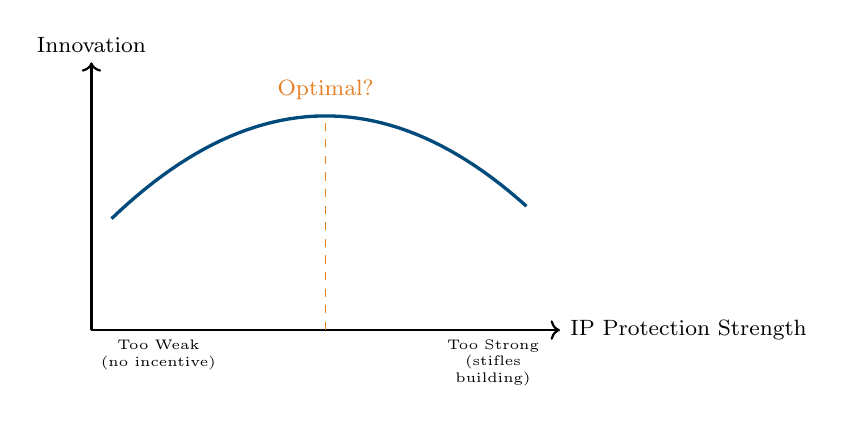
\begin{tikzpicture}[scale=0.85]
        % Axes
        \draw[thick, ->] (0,0) -- (7,0) node[right, font=\footnotesize] {IP Protection Strength};
        \draw[thick, ->] (0,0) -- (0,4) node[above, font=\footnotesize] {Innovation};
        
        % Inverted U curve
        \draw[very thick, primaryblue, domain=0.3:6.5, samples=50] plot (\x, {-0.15*(\x-3.5)^2 + 3.2});
        
        % Labels
        \node[below, font=\tiny, text width=1.5cm, align=center] at (1,0) {Too Weak\\(no incentive)};
        \node[below, font=\tiny, text width=1.5cm, align=center] at (6,0) {Too Strong\\(stifles building)};
        \node[above, font=\footnotesize, accentorange] at (3.5,3.3) {Optimal?};
        \draw[dashed, accentorange] (3.5,0) -- (3.5,3.2);
    \end{tikzpicture}
\end{frame}

%------------------------------------------------------
% SLIDE 8: Lockean Justifications for IP
%------------------------------------------------------
\begin{frame}{Lockean Justifications for IP}
    \begin{itemize}
        \item Philosopher John Locke argued that property rights arise when you \textbf{mix your labor} with something unowned---by working the land, you make it yours.
        \item Applied to intellectual property: when you invest mental effort to create something new---a novel, an invention, a song---the product of that labor rightfully belongs to you.
        \item Unlike the utilitarian view, this is a \textbf{natural rights} argument: you deserve the fruits of your labor regardless of whether IP laws maximize social welfare.
        \item The Lockean view explains why IP infringement feels like \textit{theft}---someone is taking what you created through your own effort.
    \end{itemize}
    
    \vspace{0.3em}
    
    \begin{exampleblock}{Locke on Labor and Property}
        ``Whatsoever then he removes out of the state that nature hath provided, and left it in, he hath mixed his labour with, and joined to it something that is his own, and thereby makes it his property.'' \\ \hfill ---John Locke, \textit{Second Treatise of Government} (1689)
    \end{exampleblock}
\end{frame}

%------------------------------------------------------
% SLIDE 9: Challenges to Lockean IP Theory
%------------------------------------------------------
\begin{frame}{Challenges to Lockean IP Theory}
    \begin{itemize}
        \item Ideas always build on previous ideas---Newton famously said he saw further by ``standing on the shoulders of giants''---so can anyone claim their creation is purely their own labor?
        \item Unlike physical property, ideas are not naturally scarce: if I ``take'' your idea, you still have it, so the usual justification for property rights (preventing deprivation) doesn't obviously apply.
        \item Locke's theory included a crucial \textbf{proviso}: you can only claim property if you leave ``enough and as good'' for others to use---but strong IP rights may violate this by restricting everyone else's access.
        \item The Lockean view also struggles to explain why IP should ever expire: if you earned it through labor, why should it enter the public domain after a set number of years?
    \end{itemize}
    
    \vspace{0.3em}
    
    \begin{alertblock}{The Lockean Proviso Problem}
        When you fence off land, others can still use different land. But when you patent an invention or copyright an expression, you restrict \textit{everyone} from using that specific idea---potentially leaving nothing ``enough and as good'' for others.
    \end{alertblock}
\end{frame}

%------------------------------------------------------
% SLIDE 10: Arguments Against Strong IP
%------------------------------------------------------
\begin{frame}{Arguments Against Strong IP}
    \begin{itemize}
        \item The slogan ``information wants to be free'' (Stewart Brand, 1984) captures the idea that IP creates \textbf{artificial scarcity} where none naturally exists---ideas can be copied infinitely at near-zero cost.
        \item Critics argue that strong IP concentrates power in large corporations rather than individual creators, since companies can afford lawyers and lobbying while artists often sign away their rights.
        \item Historical evidence is mixed: many scientific breakthroughs (from calculus to the polio vaccine) occurred without IP incentives, suggesting innovation doesn't require strong protection.
        \item Some economists argue IP actually \textit{reduces} innovation by preventing others from building on existing ideas and by encouraging secrecy over sharing.
    \end{itemize}
    
    \vspace{0.3em}
    
    \begin{exampleblock}{Jonas Salk and the Polio Vaccine}
        When asked who owned the patent on his polio vaccine, Jonas Salk replied: ``The people. Could you patent the sun?'' He deliberately chose not to patent it, allowing free global distribution that saved millions of lives.
    \end{exampleblock}
\end{frame}

%------------------------------------------------------
% SLIDE 11: Finding Balance: The IP Spectrum
%------------------------------------------------------
\begin{frame}{Finding Balance: The IP Spectrum}
    \begin{itemize}
        \item IP policy exists on a spectrum from no protection at all (everything in the public domain) to maximal protection (perpetual, absolute rights over every creation).
        \item Different societies have chosen different points on this spectrum, and the same society may choose different levels for different types of IP (stronger for pharmaceuticals, weaker for fashion).
        \item Over the past century, IP terms have consistently expanded: U.S. copyright went from 14 years (1790) to 28 years (1909) to life plus 50 years (1976) to life plus 70 years (1998).
        \item Critics call this ``term creep'' and note that each extension came just before Mickey Mouse would have entered the public domain---earning the 1998 law the nickname ``Mickey Mouse Protection Act.''
    \end{itemize}
    
    \vspace{0.3em}
    
    \centering
    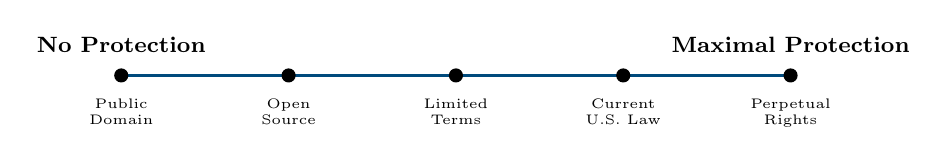
\begin{tikzpicture}[scale=0.85]
        % Spectrum line
        \draw[very thick, primaryblue] (0,0) -- (10,0);
        
        % Endpoints
        \node[above, font=\footnotesize\bfseries] at (0,0.2) {No Protection};
        \node[above, font=\footnotesize\bfseries] at (10,0.2) {Maximal Protection};
        
        % Markers
        \fill (0,0) circle (3pt);
        \fill (2.5,0) circle (3pt);
        \fill (5,0) circle (3pt);
        \fill (7.5,0) circle (3pt);
        \fill (10,0) circle (3pt);
        
        % Labels below
        \node[below, font=\tiny, text width=1.8cm, align=center] at (0,-0.2) {Public\\Domain};
        \node[below, font=\tiny, text width=1.8cm, align=center] at (2.5,-0.2) {Open\\Source};
        \node[below, font=\tiny, text width=1.8cm, align=center] at (5,-0.2) {Limited\\Terms};
        \node[below, font=\tiny, text width=1.8cm, align=center] at (7.5,-0.2) {Current\\U.S. Law};
        \node[below, font=\tiny, text width=1.8cm, align=center] at (10,-0.2) {Perpetual\\Rights};
    \end{tikzpicture}
\end{frame}

%------------------------------------------------------
% SLIDE 12: Discussion Questions: Philosophy of IP
%------------------------------------------------------
\begin{frame}{Discussion Questions: Philosophy of IP}
    \begin{enumerate}
        \item If you write a song, do you ``own'' the melody the way you own your bicycle? What's similar about these two types of ownership, and what's fundamentally different?
        
        \vspace{0.5em}
        
        \item The utilitarian view says IP is justified if it maximizes innovation. What kind of evidence would show that current IP terms are too long---or too short?
        
        \vspace{0.5em}
        
        \item The Lockean view says you own what you create through your labor. But if all ideas build on previous ideas, can anyone truly claim original ownership of their creations?
        
        \vspace{0.5em}
        
        \item Jonas Salk gave away the polio vaccine freely. Should more inventors follow his example? What would happen to pharmaceutical research if no one could patent medicines?
    \end{enumerate}
\end{frame}

%------------------------------------------------------
% SLIDE 13: Patents: Protecting Inventions
%------------------------------------------------------
\begin{frame}{Patents: Protecting Inventions}
    \begin{itemize}
        \item A \textbf{patent} grants the inventor exclusive rights to make, use, and sell an invention for a limited time---typically 20 years from the filing date in most countries.
        \item To receive a patent, an invention must meet three requirements: it must be \textbf{novel} (new), \textbf{non-obvious} (not an evident next step), and \textbf{useful} (it actually works).
        \item In exchange for this temporary monopoly, the inventor must \textbf{publicly disclose} how the invention works, adding to humanity's collective knowledge.
        \item After the patent expires, anyone can freely use the invention---this is how generic drugs become available after brand-name patents end.
    \end{itemize}
    
    \vspace{0.3em}
    
    \begin{block}{The Three Requirements for Patentability}
        \textbf{Novel}: No one has done this exact thing before. \textbf{Non-obvious}: A skilled person in the field wouldn't consider it an obvious next step. \textbf{Useful}: It actually accomplishes something practical.
    \end{block}
\end{frame}

%------------------------------------------------------
% SLIDE 14: Case Study: Pharmaceutical Patents and Public Health
%------------------------------------------------------
\begin{frame}{Case Study: Pharmaceutical Patents and Public Health}
    \begin{itemize}
        \item Developing a new drug costs an estimated \$1--2 billion and takes 10--15 years, so pharmaceutical companies argue patents are essential to recoup these massive investments.
        \item However, patent-protected drugs can cost 10--100 times more than generics, putting life-saving treatments out of reach for patients in poorer countries.
        \item The HIV/AIDS crisis made this tension visible: patented antiretroviral drugs cost \$10,000+/year while generic versions cost under \$100, leading to millions of preventable deaths.
        \item COVID-19 renewed the debate: should vaccine patents be waived during global health emergencies to allow faster, cheaper worldwide production?
    \end{itemize}
    
    \vspace{0.3em}
    
    \begin{table}[h]
        \centering
        \footnotesize
        \begin{tabular}{lrr}
            \toprule
            \textbf{Medication} & \textbf{Brand Price} & \textbf{Generic Price} \\
            \midrule
            Humira (arthritis) & \$5,800/month & \$1,200/month \\
            Sovaldi (hepatitis C) & \$1,000/pill & \$4/pill (India) \\
            Insulin (diabetes) & \$300/vial & \$25/vial (biosimilar) \\
            \bottomrule
        \end{tabular}
    \end{table}
\end{frame}

%------------------------------------------------------
% SLIDE 15: Trade Secrets: The Coca-Cola Approach
%------------------------------------------------------
\begin{frame}{Trade Secrets: The Coca-Cola Approach}
    \begin{itemize}
        \item A \textbf{trade secret} is confidential business information that provides competitive advantage---formulas, processes, customer lists, or strategies that companies keep hidden.
        \item Unlike patents, trade secrets require no registration and can last \textit{forever}---as long as the information remains secret.
        \item The law protects trade secrets against theft, espionage, and breach of confidentiality agreements, but offers no protection if someone independently discovers or reverse-engineers the secret.
        \item The risk is total loss: once a trade secret becomes public (through leaks, hacking, or carelessness), protection is gone permanently with no way to restore it.
    \end{itemize}
    
    \vspace{0.3em}
    
    \begin{exampleblock}{Coca-Cola's Famous Formula}
        Coca-Cola has kept its formula secret since 1886---over 135 years. The company chose secrecy over patents because a patent would have expired decades ago and revealed the recipe to everyone. Only two executives allegedly know the complete formula, and they're forbidden from flying on the same plane.
    \end{exampleblock}
\end{frame}

%------------------------------------------------------
% SLIDE 16: Copyright: Protecting Creative Expression
%------------------------------------------------------
\begin{frame}{Copyright: Protecting Creative Expression}
    \begin{itemize}
        \item \textbf{Copyright} protects original works of authorship---books, music, films, artwork, software code, and other creative expressions---giving creators control over reproduction, distribution, and adaptation.
        \item Copyright is \textbf{automatic}: the moment you create something original and fix it in tangible form (write it down, record it), you have copyright---no registration required.
        \item Crucially, copyright protects \textbf{expression, not ideas}: anyone can write a story about a boy wizard at magic school, but they can't copy J.K. Rowling's specific words and characters.
        \item Current U.S. copyright lasts for the author's life plus 70 years---meaning works created today won't enter the public domain until the 22nd century.
    \end{itemize}
    
    \vspace{0.3em}
    
    \begin{table}[h]
        \centering
        \footnotesize
        \begin{tabular}{p{4.5cm}p{5cm}}
            \toprule
            \textbf{Protected by Copyright} & \textbf{NOT Protected} \\
            \midrule
            Harry Potter novels (specific text) & Idea of wizard school story \\
            ``Shape of You'' recording & Basic chord progressions \\
            Windows source code & Concept of operating system \\
            Photograph you took & Facts depicted in photo \\
            \bottomrule
        \end{tabular}
    \end{table}
\end{frame}

%------------------------------------------------------
% SLIDE 17: Fair Use: When Copying Is Allowed
%------------------------------------------------------
\begin{frame}{Fair Use: When Copying Is Allowed}
    \begin{itemize}
        \item \textbf{Fair use} is a legal doctrine that allows limited use of copyrighted material without permission for purposes like criticism, commentary, news reporting, teaching, and research.
        \item Courts evaluate fair use by weighing four factors: the purpose of the use, the nature of the original work, how much was taken, and the effect on the market for the original.
        \item Fair use is deliberately flexible---there are no bright-line rules, which means each case depends on its specific facts and requires judgment.
        \item This flexibility protects free expression but creates uncertainty: you often can't know for sure whether something is fair use until a court decides.
    \end{itemize}
    
    \vspace{0.3em}
    
    \begin{block}{The Four Fair Use Factors}
        \textbf{1. Purpose}: Commercial or educational? Transformative? \textbf{2. Nature}: Factual works get less protection than creative ones. \textbf{3. Amount}: How much was used relative to the whole? \textbf{4. Market Effect}: Does it substitute for the original?
    \end{block}
\end{frame}

%------------------------------------------------------
% SLIDE 18: Fair Use in Practice
%------------------------------------------------------
\begin{frame}{Fair Use in Practice}
    \begin{itemize}
        \item \textbf{Parody} is generally protected: ``Weird Al'' Yankovic's song parodies mock the originals, transforming them into comedy (though he asks permission anyway out of courtesy).
        \item \textbf{Commentary and criticism} often qualify: video essayists can use film clips to analyze and critique movies because the clips serve a new purpose.
        \item \textbf{Transformative use} is key: appropriation artists like Andy Warhol took existing images but transformed their meaning---courts increasingly favor uses that add new expression or meaning.
        \item \textbf{Educational use} has some protection, but it's not absolute: showing a film in class may be fair use, but photocopying an entire textbook for students is not.
    \end{itemize}
    
    \vspace{0.3em}
    
    \begin{exampleblock}{Campbell v. Acuff-Rose (1994)}
        2 Live Crew's rap parody of Roy Orbison's ``Pretty Woman'' was ruled fair use by the Supreme Court, even though it was commercial and used the song's distinctive opening riff. The Court held that parody is transformative because it comments on the original work.
    \end{exampleblock}
\end{frame}

%------------------------------------------------------
% SLIDE 19: Trademarks: Protecting Brands
%------------------------------------------------------
\begin{frame}{Trademarks: Protecting Brands}
    \begin{itemize}
        \item A \textbf{trademark} is a word, symbol, design, or combination that identifies the source of goods or services---the Nike swoosh, McDonald's golden arches, or Apple's apple.
        \item Trademarks protect consumers from confusion (ensuring you get authentic products) and protect businesses' investment in their reputation and brand identity.
        \item Unlike patents and copyrights, trademarks can last \textit{forever}---as long as the owner continues using and actively defending the mark.
        \item Companies must aggressively protect trademarks or risk \textbf{genericide}: when a brand name becomes so common it loses protection (aspirin, escalator, thermos, zipper were all once trademarks).
    \end{itemize}
    
    \vspace{0.3em}
    
    \begin{alertblock}{Why Companies Seem Trademark-Obsessed}
        When Google asks you to say ``search the web'' instead of ``google it,'' they're not being petty---they're trying to prevent ``google'' from becoming generic like ``xerox'' or ``kleenex.'' Losing trademark status means losing exclusive rights to your own brand name.
    \end{alertblock}
\end{frame}

%------------------------------------------------------
% SLIDE 20: Comparing Intellectual Property Types
%------------------------------------------------------
\begin{frame}{Comparing Intellectual Property Types}
    \begin{center}
    \footnotesize
    \renewcommand{\arraystretch}{1.2}
    \begin{tabular}{>{\raggedright}p{1.8cm} >{\raggedright}p{2.2cm} >{\raggedright}p{2.2cm} >{\raggedright}p{1.8cm} >{\raggedright\arraybackslash}p{2.5cm}}
        \toprule
        \textbf{Type} & \textbf{What It Protects} & \textbf{Duration} & \textbf{Registration} & \textbf{Example} \\
        \midrule
        Patent & Inventions, processes & 20 years & Required & iPhone touch screen \\
        \addlinespace
        Copyright & Creative expression & Life + 70 years & Automatic & \textit{Harry Potter} novels \\
        \addlinespace
        Trademark & Brand identifiers & Forever (if used) & Recommended & Nike swoosh \\
        \addlinespace
        Trade Secret & Confidential info & While secret & None & Coca-Cola formula \\
        \bottomrule
    \end{tabular}
    \end{center}
    
    \vspace{0.3em}
    
    \begin{block}{Choosing the Right Protection}
        The same product might involve multiple IP types: a smartphone includes patented technology, copyrighted software, trademarked logos, and trade secret manufacturing processes. Companies strategically combine protections.
    \end{block}
\end{frame}

%------------------------------------------------------
% SLIDE 21: Case Study: The Smartphone Patent Wars
%------------------------------------------------------
\begin{frame}{Case Study: The Smartphone Patent Wars}
    \begin{itemize}
        \item When Apple launched the iPhone in 2007, Steve Jobs declared he would use ``thermonuclear war'' to destroy Android, which he viewed as a stolen product---launching years of patent litigation.
        \item Apple sued Samsung for copying the iPhone's design, including its rounded rectangular shape, grid of icons, and slide-to-unlock feature, winning over \$1 billion in damages (later reduced).
        \item Critics argued these patents covered obvious design choices that no one should own: rectangles with rounded corners have existed for centuries, and grid layouts are a natural way to organize apps.
        \item The wars eventually cooled as companies realized mutual destruction was costly, but the episode showed how patent systems can be weaponized against competitors.
    \end{itemize}
    
    \vspace{0.3em}
    
    \begin{block}{Patents at Issue in Apple v. Samsung}
        \textbf{Design patents}: Rounded rectangle shape, icon grid layout, home button placement. \textbf{Utility patents}: Pinch-to-zoom, bounce-back scrolling, slide-to-unlock. Samsung argued these were either obvious or features Android developed independently.
    \end{block}
\end{frame}

%------------------------------------------------------
% SLIDE 22: Case Study: Music Sampling and "Blurred Lines"
%------------------------------------------------------
\begin{frame}{Case Study: Music Sampling and ``Blurred Lines''}
    \begin{itemize}
        \item \textbf{Sampling}---using pieces of existing recordings in new songs---has been central to hip-hop and electronic music since the 1980s, but copyright law has made it increasingly risky.
        \item In \textit{Bridgeport Music v. Dimension Films} (2005), the court ruled that even a two-second, unrecognizable sample requires a license, declaring ``get a license or do not sample.''
        \item The ``Blurred Lines'' case (2015) went further: Robin Thicke and Pharrell Williams were ordered to pay \$5 million to Marvin Gaye's estate because their song captured the ``feel'' of Gaye's ``Got to Give It Up''---even without copying specific notes.
        \item Musicians and legal scholars warned this could chill creativity by making artists liable for songs that merely sound similar to older works.
    \end{itemize}
    
    \vspace{0.3em}
    
    \begin{alertblock}{From the Dissent}
        ``The majority allows the Gaye family to accomplish what no one has before: copyright a musical style... Blurred Lines and Got to Give It Up are not objectively similar. They differ in melody, harmony, and rhythm.'' The dissent warned this ruling would ``strike a devastating blow'' to creativity.
    \end{alertblock}
\end{frame}

%------------------------------------------------------
% SLIDE 23: Patent Trolls and IP Abuse
%------------------------------------------------------
\begin{frame}{Patent Trolls and IP Abuse}
    \begin{itemize}
        \item \textbf{Patent trolls} (or ``non-practicing entities'') are companies that acquire patents not to make products but solely to sue or threaten others for infringement.
        \item Their business model exploits the fact that patent litigation costs millions to defend, so many companies pay settlements even for dubious claims rather than fight in court.
        \item Small businesses and startups are particularly vulnerable: a troll's demand letter can threaten their survival, forcing them to pay ``licensing fees'' for patents they may not even infringe.
        \item Studies estimate patent trolls cost the U.S. economy \$29 billion annually in direct costs, plus immeasurable innovation lost when startups shut down or avoid certain technologies.
    \end{itemize}
    
    \vspace{0.3em}
    
    \begin{exampleblock}{A Notorious Example}
        The company Lodsys sued dozens of small app developers for using in-app purchase buttons, claiming to own a patent on the concept. Many developers couldn't afford lawyers and either paid up or removed their apps entirely---even though Apple had already licensed the underlying technology.
    \end{exampleblock}
\end{frame}

%------------------------------------------------------
% SLIDE 24: Discussion Questions: Types of IP
%------------------------------------------------------
\begin{frame}{Discussion Questions: Types of IP}
    \begin{enumerate}
        \item Pharmaceutical patents let companies charge high prices to recoup R\&D costs, but this puts medicines out of reach for many. How should we balance innovation incentives against access to life-saving drugs?
        
        \vspace{0.5em}
        
        \item Copyright currently lasts for the author's life plus 70 years. Is this too long, too short, or about right? What would be your ideal copyright term, and why?
        
        \vspace{0.5em}
        
        \item The ``Blurred Lines'' verdict found infringement based on a song's ``feel'' rather than copied notes. Should musical style or groove be protectable? Where would you draw the line?
        
        \vspace{0.5em}
        
        \item Amazon patented ``one-click purchasing.'' Should software features and business methods be patentable, or should patents be limited to physical inventions?
    \end{enumerate}
\end{frame}

%------------------------------------------------------
% SLIDE 25: The DMCA: America's Digital Copyright Law
%------------------------------------------------------
\begin{frame}{The DMCA: America's Digital Copyright Law}
    \begin{itemize}
        \item The \textbf{Digital Millennium Copyright Act (DMCA)}, passed in 1998, was designed to update copyright law for the internet age---when Napster and MP3 sharing were revolutionizing how people accessed music.
        \item The law has two major components: \textbf{safe harbor} provisions that protect platforms from liability for user uploads, and \textbf{anti-circumvention} rules that make it illegal to bypass digital locks.
        \item Originally focused on music and movie piracy, the DMCA now affects nearly every digital technology---from YouTube videos to smart tractors to medical devices.
        \item Critics argue the law has expanded far beyond its original purpose, giving copyright holders powerful tools that can be used to suppress competition, criticism, and repair.
    \end{itemize}
    
    \vspace{0.3em}
    
    \begin{block}{The Two Pillars of the DMCA}
        \textbf{Safe Harbors (§512)}: Platforms aren't liable for user content if they respond to takedown notices. \textbf{Anti-Circumvention (§1201)}: Breaking digital locks is illegal, even if your intended use would otherwise be lawful.
    \end{block}
\end{frame}

%------------------------------------------------------
% SLIDE 26: DMCA Safe Harbors and Notice-and-Takedown
%------------------------------------------------------
\begin{frame}{DMCA Safe Harbors and Notice-and-Takedown}
    \begin{itemize}
        \item The safe harbor system enabled the modern internet: without it, platforms like YouTube, Facebook, and Reddit would be liable for every infringing post by every user---an impossible burden.
        \item In exchange for immunity, platforms must respond to \textbf{takedown notices} from copyright holders by promptly removing allegedly infringing content.
        \item Users can file a \textbf{counter-notice} claiming their use was lawful; if the copyright holder doesn't sue within 14 days, the content goes back up.
        \item The system processes millions of takedowns yearly---Google alone receives over 5 million URL removal requests per week.
    \end{itemize}
    
    \vspace{0.3em}
    
    \centering
    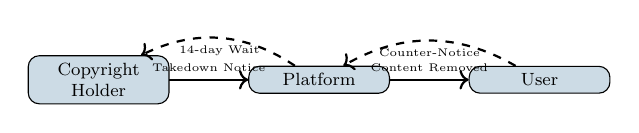
\begin{tikzpicture}[scale=0.8, transform shape]
        \node[draw, rounded corners, fill=primaryblue!20, text width=2cm, align=center, font=\footnotesize] at (0,0) (holder) {Copyright\\Holder};
        \node[draw, rounded corners, fill=primaryblue!20, text width=2cm, align=center, font=\footnotesize] at (3.5,0) (platform) {Platform};
        \node[draw, rounded corners, fill=primaryblue!20, text width=2cm, align=center, font=\footnotesize] at (7,0) (user) {User};
        
        \draw[->, thick] (holder) -- (platform) node[midway, above, font=\tiny] {Takedown Notice};
        \draw[->, thick] (platform) -- (user) node[midway, above, font=\tiny] {Content Removed};
        \draw[->, thick, dashed] (user) to[bend right=30] node[midway, below, font=\tiny] {Counter-Notice} (platform);
        \draw[->, thick, dashed] (platform) to[bend right=30] node[midway, below, font=\tiny] {14-day Wait} (holder);
    \end{tikzpicture}
\end{frame}

%------------------------------------------------------
% SLIDE 27: Case Study: YouTube, Content ID, and Creators
%------------------------------------------------------
\begin{frame}{Case Study: YouTube, Content ID, and Creators}
    \begin{itemize}
        \item YouTube's \textbf{Content ID} system automatically scans every upload against a database of copyrighted material, allowing rights holders to block, monetize, or track matching content.
        \item Content ID processes over 500 years' worth of video daily and has paid rights holders over \$9 billion---but creators complain the system is prone to abuse and errors.
        \item \textbf{False positives} are common: birdsong has been flagged as copyrighted music, white noise videos have received claims, and public domain classical recordings are routinely blocked.
        \item The system doesn't recognize fair use, so video essayists, educators, and critics often have legitimate content blocked or demonetized with no easy way to appeal.
    \end{itemize}
    
    \vspace{0.3em}
    
    \begin{alertblock}{When Algorithms Decide Fair Use}
        A music theory channel analyzing a pop song, a film critic reviewing a movie, a teacher explaining a poem---all may have their videos claimed by Content ID. The algorithm can't tell the difference between piracy and commentary.
    \end{alertblock}
\end{frame}

%------------------------------------------------------
% SLIDE 28: DMCA Anti-Circumvention: Breaking Digital Locks
%------------------------------------------------------
\begin{frame}{DMCA Anti-Circumvention: Breaking Digital Locks}
    \begin{itemize}
        \item Section 1201 of the DMCA makes it illegal to circumvent \textbf{technological protection measures} (TPMs)---the digital locks, encryption, and DRM that control access to copyrighted content.
        \item The twist: breaking these locks is illegal \textit{even if your intended use would be perfectly legal}, such as making a backup copy, exercising fair use rights, or accessing content you purchased.
        \item This means you can legally own a DVD but face federal penalties for bypassing its copy protection to watch it on your laptop without a DVD drive.
        \item The law also prohibits distributing circumvention tools, making it difficult for legitimate researchers to share security findings or for consumers to access repair information.
    \end{itemize}
    
    \vspace{0.3em}
    
    \begin{exampleblock}{The Paradox of Legal Uses Made Illegal}
        Making a personal backup of a movie you bought: \textit{Legal}. Breaking the DRM to make that backup: \textit{Federal crime}. The DMCA criminalizes the means to exercise rights you otherwise have.
    \end{exampleblock}
\end{frame}

%------------------------------------------------------
% SLIDE 29: DMCA and Gaming: Emulation and Preservation
%------------------------------------------------------
\begin{frame}{DMCA and Gaming: Emulation and Preservation}
    \begin{itemize}
        \item \textbf{Emulators} are software programs that mimic old game consoles, allowing you to play classic games on modern computers---the emulator itself is generally legal under \textit{Sony v. Connectix} (2000).
        \item \textbf{ROMs}---the game files themselves---exist in legal gray area: making a backup of a game you own may be legal, but downloading ROMs online is typically copyright infringement.
        \item Video game preservation faces a crisis: thousands of classic games are becoming unplayable as old hardware dies and companies refuse to re-release titles, yet preserving them may violate the DMCA.
        \item The Library of Congress has granted limited DMCA exemptions for game preservation, but they're narrow and require re-approval every three years.
    \end{itemize}
    
    \vspace{0.3em}
    
    \begin{table}[h]
        \centering
        \footnotesize
        \begin{tabular}{lc}
            \toprule
            \textbf{Activity} & \textbf{Legal Status} \\
            \midrule
            Creating/using an emulator & Generally legal \\
            Dumping ROM from cartridge you own & Likely legal \\
            Downloading ROMs online & Usually infringement \\
            Breaking DRM to preserve games & DMCA violation \\
            \bottomrule
        \end{tabular}
    \end{table}
\end{frame}

%------------------------------------------------------
% SLIDE 30: Case Study: Nintendo vs. Fan Games and ROMs
%------------------------------------------------------
\begin{frame}{Case Study: Nintendo vs. Fan Games and ROMs}
    \begin{itemize}
        \item Nintendo aggressively pursues any unauthorized use of its intellectual property, sending cease-and-desist letters to fan game creators, ROM sites, and even people selling used games.
        \item Fan-made projects like \textbf{AM2R} (a Metroid remake) and \textbf{Pokemon Uranium} were shut down despite years of free labor by devoted fans who wanted to celebrate Nintendo's games.
        \item In 2018, Nintendo forced major ROM sites like EmuParadise and LoveROMs offline; in 2023, Gary Bowser was sentenced to 40 months in prison and ordered to pay \$10 million for selling Switch piracy tools.
        \item Preservationists argue Nintendo makes many classic games unavailable for purchase, leaving piracy as the only way to experience gaming history---Nintendo responds that IP protection is essential.
    \end{itemize}
    
    \vspace{0.3em}
    
    \begin{block}{Nintendo's Position vs. Preservationists}
        \textbf{Nintendo}: We must protect our IP to fund future games; unauthorized use hurts our brand. \textbf{Preservationists}: You've abandoned these games; if you won't preserve them, let us do it legally.
    \end{block}
\end{frame}

%------------------------------------------------------
% SLIDE 31: DMCA and Mods: Who Owns Player Creativity?
%------------------------------------------------------
\begin{frame}{DMCA and Mods: Who Owns Player Creativity?}
    \begin{itemize}
        \item \textbf{Mods} (modifications) are player-created additions to games---new levels, characters, graphics, or complete gameplay overhauls---that have been part of PC gaming culture for decades.
        \item The legal status of mods varies: most companies tolerate or encourage them, but the game's End User License Agreement (EULA) technically controls what's permitted.
        \item Some of gaming's biggest franchises started as mods: \textbf{Counter-Strike} began as a Half-Life mod, \textbf{DOTA} as a Warcraft III mod, and \textbf{PUBG} drew from ARMA mods.
        \item Tensions arise over \textbf{paid mods}: when Bethesda and Steam tried selling mods for Skyrim in 2015, the backlash was so fierce they reversed course within days.
    \end{itemize}
    
    \vspace{0.3em}
    
    \begin{exampleblock}{From Mod to Billion-Dollar Franchise}
        Defense of the Ancients (DOTA) was a free mod for Warcraft III created by anonymous modders. It spawned an entire genre (MOBA), and DOTA 2---now owned by Valve---has paid out over \$300 million in esports prizes. The original modders received nothing.
    \end{exampleblock}
\end{frame}

%------------------------------------------------------
% SLIDE 32: DMCA Everywhere: Tractors, Printers, and Cars
%------------------------------------------------------
\begin{frame}{DMCA Everywhere: Tractors, Printers, and Cars}
    \begin{itemize}
        \item The DMCA's anti-circumvention rules now reach far beyond entertainment: any product with software can use digital locks to control how owners use, modify, or repair their own property.
        \item \textbf{John Deere tractors} contain software that prevents farmers from repairing their own equipment, forcing them to pay dealer rates or wait days for authorized technicians during critical harvest windows.
        \item \textbf{Printer manufacturers} use DRM chips in ink cartridges to block cheaper third-party alternatives, turning printers into ``razors'' that lock you into expensive proprietary ``blades.''
        \item \textbf{Cars} increasingly restrict access to diagnostic software, \textbf{medical devices} prevent hospitals from servicing their own equipment, and even \textbf{cat litter boxes} have used DRM.
    \end{itemize}
    
    \vspace{0.3em}
    
    \begin{table}[h]
        \centering
        \footnotesize
        \begin{tabular}{ll}
            \toprule
            \textbf{Product} & \textbf{DRM Restriction} \\
            \midrule
            John Deere tractors & Can't access repair diagnostics \\
            HP printers & Block third-party ink cartridges \\
            Tesla vehicles & Software-locked features, repair limits \\
            Philips CPAP machines & Prescription required for settings \\
            \bottomrule
        \end{tabular}
    \end{table}
\end{frame}

%------------------------------------------------------
% SLIDE 33: The Right to Repair Movement
%------------------------------------------------------
\begin{frame}{The Right to Repair Movement}
    \begin{itemize}
        \item The \textbf{right to repair movement} is a coalition of farmers, mechanics, technicians, and consumers demanding the legal right to fix products they own without manufacturer restrictions.
        \item Advocates argue that ownership should mean repair rights, that manufacturer restrictions create unnecessary electronic waste, and that rural communities suffer when repairs require shipping equipment to distant service centers.
        \item Opponents---primarily manufacturers---argue that unrestricted repair access raises safety concerns, exposes trade secrets, and could lead to liability issues if untrained people damage products.
        \item Several U.S. states (Massachusetts, New York, Minnesota, California) have passed right to repair laws, and the FTC has signaled support for broader federal action.
    \end{itemize}
    
    \vspace{0.3em}
    
    \begin{block}{Key Arguments in the Repair Debate}
        \textbf{For}: You bought it, you own it; reduces e-waste; supports local repair shops; lowers costs. \textbf{Against}: Safety risks from improper repairs; protects trade secrets; ensures quality control; liability concerns.
    \end{block}
\end{frame}

%------------------------------------------------------
% SLIDE 34: International IP: WIPO and Global Treaties
%------------------------------------------------------
\begin{frame}{International IP: WIPO and Global Treaties}
    \begin{itemize}
        \item The \textbf{World Intellectual Property Organization (WIPO)} is a United Nations agency that coordinates international IP treaties and helps countries develop IP systems.
        \item The \textbf{TRIPS Agreement} (1995) established minimum IP standards for all World Trade Organization members, requiring countries to protect patents, copyrights, and trademarks to participate in global trade.
        \item IP enforcement varies dramatically worldwide: some countries aggressively protect IP, while others have weaker enforcement or different cultural attitudes toward copying.
        \item Critics argue that international IP rules often favor wealthy nations and large corporations, locking developing countries out of technologies they need for healthcare, education, and development.
    \end{itemize}
    
    \vspace{0.3em}
    
    \begin{table}[h]
        \centering
        \footnotesize
        \begin{tabular}{lll}
            \toprule
            \textbf{Region} & \textbf{IP Approach} & \textbf{Key Characteristic} \\
            \midrule
            United States & Very strong & Long terms, broad patents \\
            European Union & Strong & Moral rights emphasis \\
            China & Strengthening & Historically weak enforcement \\
            India & Moderate & Compulsory licensing for meds \\
            \bottomrule
        \end{tabular}
    \end{table}
\end{frame}

%------------------------------------------------------
% SLIDE 35: Case Study: DMCA Abuse and False Takedowns
%------------------------------------------------------
\begin{frame}{Case Study: DMCA Abuse and False Takedowns}
    \begin{itemize}
        \item The DMCA's notice-and-takedown system is easily abused because filing a takedown is free, fast, and carries almost no penalty for false claims.
        \item Bad actors use false takedowns to \textbf{silence critics} (removing negative reviews), \textbf{censor journalism} (taking down unflattering news stories), and \textbf{sabotage competitors} (disrupting rival businesses).
        \item \textbf{Copyfraud} occurs when people falsely claim copyright over public domain works---stock photo companies have demanded payment for photos of the Eiffel Tower at night and NASA space images.
        \item In \textit{Lenz v. Universal} (the ``Dancing Baby'' case), a court ruled that copyright holders must consider fair use before sending takedowns---but enforcement remains rare.
    \end{itemize}
    
    \vspace{0.3em}
    
    \begin{alertblock}{The Asymmetry Problem}
        Filing a false takedown: free, instant, rarely punished. Fighting a false takedown: requires legal knowledge, takes weeks, risks lawsuit. This imbalance encourages abuse and chills legitimate speech.
    \end{alertblock}
\end{frame}

%------------------------------------------------------
% SLIDE 36: Discussion Questions: DMCA and Digital Rights
%------------------------------------------------------
\begin{frame}{Discussion Questions: DMCA and Digital Rights}
    \begin{enumerate}
        \item You buy a tractor, but software locks prevent you from repairing it yourself. Should the law protect your right to repair things you legally own, even if it means breaking digital locks?
        
        \vspace{0.5em}
        
        \item YouTube's Content ID makes mistakes but processes millions of claims that would overwhelm human reviewers. Is automated copyright enforcement acceptable if it's the only way platforms can exist?
        
        \vspace{0.5em}
        
        \item Many classic video games are unplayable because companies won't re-release them and block preservation efforts. Should copyright law include stronger exceptions for preserving cultural works?
        
        \vspace{0.5em}
        
        \item DMCA takedowns are easy to file but hard to challenge. How would you reform the system to prevent abuse while still protecting copyright holders?
    \end{enumerate}
\end{frame}

%------------------------------------------------------
% SLIDE 37: What Is Open Source?
%------------------------------------------------------
\begin{frame}{What Is Open Source?}
    \begin{itemize}
        \item \textbf{Open source software} makes its source code freely available for anyone to view, modify, and distribute---in contrast to ``proprietary'' software where the code is kept secret.
        \item Open source is not necessarily free in price (companies can sell it), but it guarantees \textbf{freedoms}: to study how it works, to modify it for your needs, and to share it with others.
        \item Far from being a fringe movement, open source powers most of the modern internet: Linux runs most web servers, Android phones, and supercomputers; Apache and Nginx serve most websites.
        \item Major tech companies including Google, Microsoft, Meta, and Amazon actively contribute to open source projects, having realized that collaboration often beats secrecy.
    \end{itemize}
    
    \vspace{0.3em}
    
    \begin{block}{The Core Freedoms of Open Source}
        \textbf{Use}: Run the software for any purpose. \textbf{Study}: Examine and learn from the source code. \textbf{Modify}: Change the software to suit your needs. \textbf{Share}: Distribute copies, modified or not.
    \end{block}
\end{frame}

%------------------------------------------------------
% SLIDE 38: The Philosophy: "Free as in Freedom"
%------------------------------------------------------
\begin{frame}{The Philosophy: ``Free as in Freedom''}
    \begin{itemize}
        \item Programmer and activist \textbf{Richard Stallman} argues that software freedom is an ethical issue: proprietary software that hides its code treats users as prisoners rather than participants.
        \item Stallman distinguishes ``free software'' from ``freeware'': the point isn't zero cost but \textbf{liberty}---``free as in freedom, not free as in beer.''
        \item On this view, sharing software is a social good, and restrictions on sharing are antisocial---just as it would be wrong to forbid lending books to friends.
        \item Stallman's Free Software Foundation promotes software that respects user freedom and opposes DRM, software patents, and proprietary formats that lock users in.
    \end{itemize}
    
    \vspace{0.3em}
    
    \begin{quote}
        \footnotesize
        ``Free software is a matter of liberty, not price. To understand the concept, you should think of free as in free speech, not as in free beer.'' \\ \hfill ---Richard Stallman
    \end{quote}
\end{frame}

%------------------------------------------------------
% SLIDE 39: Key Figures: Stallman, Torvalds, and Raymond
%------------------------------------------------------
\begin{frame}{Key Figures: Stallman, Torvalds, and Raymond}
    \begin{itemize}
        \item \textbf{Richard Stallman} launched the GNU Project (1983) and Free Software Foundation, created the GPL license, and views software freedom as a moral imperative.
        \item \textbf{Linus Torvalds} created Linux (1991), the kernel that combined with GNU tools to form a complete operating system; he takes a pragmatic rather than ideological approach.
        \item \textbf{Eric Raymond} wrote ``The Cathedral and the Bazaar'' (1997), arguing that open source produces better software through decentralized collaboration---``given enough eyeballs, all bugs are shallow.''
        \item The movement split between ``free software'' (Stallman's ethical focus) and ``open source'' (Raymond's practical focus), though the licenses and code overlap significantly.
    \end{itemize}
    
    \vspace{0.3em}
    
    \begin{table}[h]
        \centering
        \footnotesize
        \begin{tabular}{lll}
            \toprule
            \textbf{Figure} & \textbf{Approach} & \textbf{Key Contribution} \\
            \midrule
            Richard Stallman & Ethical/ideological & GNU, GPL, FSF \\
            Linus Torvalds & Pragmatic/technical & Linux kernel \\
            Eric Raymond & Business/practical & Open source methodology \\
            \bottomrule
        \end{tabular}
    \end{table}
\end{frame}

%------------------------------------------------------
% SLIDE 40: Case Study: Linux vs. Windows
%------------------------------------------------------
\begin{frame}{Case Study: Linux vs. Windows}
    \begin{itemize}
        \item \textbf{Linux} is free, open source, and developed by a global community of volunteers and companies; \textbf{Windows} is proprietary, costs money, and is controlled entirely by Microsoft.
        \item Linux dominates servers (96\% of top web servers), supercomputers (100\% of top 500), cloud infrastructure, and powers every Android phone---but has only about 4\% of desktop users.
        \item Windows dominates desktops (72\%) because it came pre-installed on PCs, has more consumer software, and is what most people learned first---network effects lock users in.
        \item The comparison illustrates that ``better'' technology doesn't always win: convenience, familiarity, and ecosystem often matter more than cost, freedom, or technical merit.
    \end{itemize}
    
    \vspace{0.3em}
    
    \begin{table}[h]
        \centering
        \footnotesize
        \begin{tabular}{lcc}
            \toprule
            \textbf{Factor} & \textbf{Linux} & \textbf{Windows} \\
            \midrule
            Cost & Free & \$100--200+ \\
            Source code & Open & Proprietary \\
            Desktop market share & $\sim$4\% & $\sim$72\% \\
            Server market share & $\sim$96\% & $\sim$4\% \\
            Control & Community & Microsoft \\
            \bottomrule
        \end{tabular}
    \end{table}
\end{frame}

%------------------------------------------------------
% SLIDE 41: Open Source Licenses: Copyleft and Permissive
%------------------------------------------------------
\begin{frame}{Open Source Licenses: Copyleft and Permissive}
    \begin{itemize}
        \item Open source software still uses copyright---but instead of restricting use, open source \textbf{licenses} grant freedoms while setting conditions for how code can be shared.
        \item \textbf{Copyleft} licenses like the GPL require that any modified version also be released as open source---the freedom is ``viral,'' ensuring derivatives stay free.
        \item \textbf{Permissive} licenses like MIT and Apache allow code to be used in proprietary products without requiring the result to be open source---maximum flexibility for developers.
        \item License choice reflects philosophy and strategy: copyleft ensures a growing commons of free software, while permissive licenses encourage wider adoption by businesses.
    \end{itemize}
    
    \vspace{0.3em}
    
    \centering
    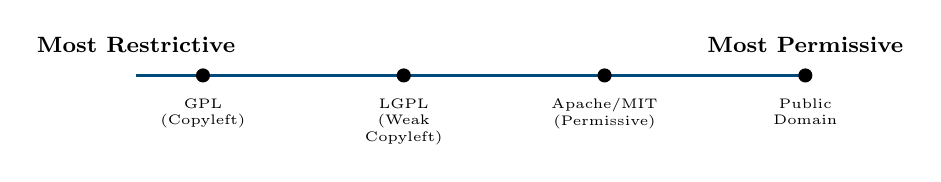
\begin{tikzpicture}[scale=0.85]
        % Spectrum line
        \draw[very thick, primaryblue] (0,0) -- (10,0);
        
        % Labels
        \node[above, font=\footnotesize\bfseries] at (0,0.2) {Most Restrictive};
        \node[above, font=\footnotesize\bfseries] at (10,0.2) {Most Permissive};
        
        % Points
        \fill (1,0) circle (3pt);
        \node[below, font=\tiny, text width=1.5cm, align=center] at (1,-0.2) {GPL\\(Copyleft)};
        \fill (4,0) circle (3pt);
        \node[below, font=\tiny, text width=1.5cm, align=center] at (4,-0.2) {LGPL\\(Weak Copyleft)};
        \fill (7,0) circle (3pt);
        \node[below, font=\tiny, text width=1.5cm, align=center] at (7,-0.2) {Apache/MIT\\(Permissive)};
        \fill (10,0) circle (3pt);
        \node[below, font=\tiny, text width=1.5cm, align=center] at (10,-0.2) {Public\\Domain};
    \end{tikzpicture}
\end{frame}

%------------------------------------------------------
% SLIDE 42: Creative Commons: Open Licensing Beyond Software
%------------------------------------------------------
\begin{frame}{Creative Commons: Open Licensing Beyond Software}
    \begin{itemize}
        \item \textbf{Creative Commons (CC)} provides standardized licenses for creative works---text, images, music, video---allowing creators to share while keeping some rights.
        \item CC licenses use mix-and-match conditions: \textbf{Attribution (BY)} requires credit; \textbf{ShareAlike (SA)} requires derivatives use the same license; \textbf{NonCommercial (NC)} prohibits commercial use; \textbf{NoDerivatives (ND)} prohibits modifications.
        \item Wikipedia, Khan Academy, many textbooks, and millions of Flickr photos use Creative Commons licenses, creating a vast pool of legally shareable educational content.
        \item The most open option, \textbf{CC0}, dedicates work to the public domain, waiving all rights---while the most restrictive (CC BY-NC-ND) allows only sharing with attribution.
    \end{itemize}
    
    \vspace{0.3em}
    
    \begin{table}[h]
        \centering
        \footnotesize
        \begin{tabular}{lcccl}
            \toprule
            \textbf{License} & \textbf{Credit} & \textbf{Commercial} & \textbf{Modify} & \textbf{Example Use} \\
            \midrule
            CC BY & Required & Yes & Yes & Wikipedia \\
            CC BY-SA & Required & Yes & Yes (share alike) & OpenStax textbooks \\
            CC BY-NC & Required & No & Yes & Educational blogs \\
            CC0 & No & Yes & Yes & Public domain dedication \\
            \bottomrule
        \end{tabular}
    \end{table}
\end{frame}

%------------------------------------------------------
% SLIDE 43: Open vs. Closed AI Models
%------------------------------------------------------
\begin{frame}{Open vs. Closed AI Models}
    \begin{itemize}
        \small
        \item \textbf{Closed AI models} like OpenAI's GPT, Anthropic's Claude, and Google's Gemini keep their weights secret---you can only access them through APIs controlled by the company, which sets rules and prices.
        \item \textbf{Open AI models} release weights publicly, allowing anyone to download, run locally, modify, and build upon them---examples include Meta's LLaMA, France's Mistral, and China's Qwen and DeepSeek.
        \item Many leading open models are now \textbf{Chinese-developed}, which raises distinct concerns: built-in censorship of politically sensitive topics, potential alignment with Chinese government interests, and uncertainty about training data sources.
        \item Ironically, \textbf{OpenAI}---founded in 2015 to develop AI ``for the benefit of all humanity''---has become increasingly closed, citing safety and competitive concerns as Chinese alternatives proliferate.
    \end{itemize}
    
    \vspace{0.3em}
    
    \begin{alertblock}{Open Models, New Questions}
        Open models enable transparency and prevent Western corporate monopolies---but what if the leading open models come with Chinese government censorship baked in? ``Open'' doesn't necessarily mean ``free from control.''
    \end{alertblock}
\end{frame}

%------------------------------------------------------
% SLIDE 44: Discussion Questions: Open Source and Open Culture
%------------------------------------------------------
\begin{frame}{Discussion Questions: Open Source and Open Culture}
    \begin{enumerate}
        \item Linux is free and dominates servers, yet most people pay for Windows on their desktops. Why do you think this is? What would it take for open source to win on the desktop?
        
        \vspace{0.5em}
        
        \item Should powerful AI models be open source so anyone can inspect and modify them? What are the benefits and risks of releasing AI weights to the public?
        
        \vspace{0.5em}
        
        \item Richard Stallman argues that proprietary software is unethical because it restricts user freedom. Do you agree, or is closed-source software just a legitimate business choice?
        
        \vspace{0.5em}
        
        \item If you created something valuable---software, music, writing---would you release it under an open license? What factors would influence your decision?
    \end{enumerate}
\end{frame}

%------------------------------------------------------
% SLIDE 45: How AI Models Learn: The Training Data Question
%------------------------------------------------------
\begin{frame}{How AI Models Learn: The Training Data Question}
    \begin{itemize}
        \item Large language models like GPT and Claude are trained on \textbf{billions of web pages, books, and articles}---a dataset equivalent to trillions of words, or a document over 3.7 billion pages long.
        \item Image generators like Stable Diffusion, Midjourney, and DALL-E trained on \textbf{millions of images} scraped from the internet, often without permission from artists or photographers.
        \item Most of this training data was used without explicit consent from creators---companies argue consent isn't required, while creators say their work was stolen.
        \item The scale is unprecedented: no human could read or view even a tiny fraction of what AI models have absorbed, making traditional copyright concepts difficult to apply.
    \end{itemize}
    
    \vspace{0.3em}
    
    \begin{block}{What's in the Training Data?}
        Common sources include: \textbf{Common Crawl} (petabytes of web pages), \textbf{Books3/LibGen} (hundreds of thousands of pirated books), \textbf{LAION} (5 billion images), and proprietary datasets scraped from news sites, social media, and code repositories.
    \end{block}
\end{frame}

%------------------------------------------------------
% SLIDE 46: Current Lawsuits: Creators vs. AI Companies
%------------------------------------------------------
\begin{frame}{Current Lawsuits: Creators vs. AI Companies}
    \begin{itemize}
        \item As of late 2025, over \textbf{50 copyright lawsuits} have been filed against AI companies, with major cases unlikely to reach final verdicts until 2026 or later.
        \item \textbf{New York Times v. OpenAI/Microsoft}: The Times alleges millions of articles were used without permission; OpenAI has been ordered to hand over internal communications about deleting training data.
        \item \textbf{Authors v. OpenAI/Anthropic}: Writers claim their books were scraped from piracy sites (``shadow libraries''); Anthropic agreed to a \$1.5 billion settlement in late 2025.
        \item \textbf{Getty Images v. Stability AI}: 12 million photographs allegedly used to train image generators; artists in \textit{Andersen v. Stability AI} raise similar claims.
    \end{itemize}
    
    \vspace{0.3em}
    
    \begin{table}[h]
        \centering
        \footnotesize
        \begin{tabular}{lll}
            \toprule
            \textbf{Plaintiff} & \textbf{Defendant} & \textbf{Core Claim} \\
            \midrule
            New York Times & OpenAI, Microsoft & Millions of articles copied \\
            Getty Images & Stability AI & 12 million photos infringed \\
            Record Labels (RIAA) & Suno, Udio & Music used to train generators \\
            Visual Artists & Midjourney, Stability & Art styles copied without consent \\
            \bottomrule
        \end{tabular}
    \end{table}
\end{frame}

%------------------------------------------------------
% SLIDE 47: The Big Questions: Fair Use, Compensation, and Society
%------------------------------------------------------
\begin{frame}{The Big Questions: Fair Use, Compensation, and Society}
    \begin{itemize}
        \item AI companies claim \textbf{fair use}: training is transformative because the AI creates new outputs, not copies; it's like a human learning from books they've read.
        \item Creators respond that AI \textbf{directly competes} with them: why hire an illustrator when Midjourney can imitate their style? Why subscribe to a newspaper when ChatGPT summarizes it?
        \item If compensation is owed, who should receive it? Individual creators whose specific works were used? All creators in a field? Society as a whole, since AI benefits from our collective knowledge?
        \item Some companies are now \textbf{licensing content} (OpenAI deals with Reddit, Associated Press, News Corp), suggesting the industry sees legal risk---but most creators have no leverage to negotiate.
    \end{itemize}
    
    \vspace{0.3em}
    
    \centering
    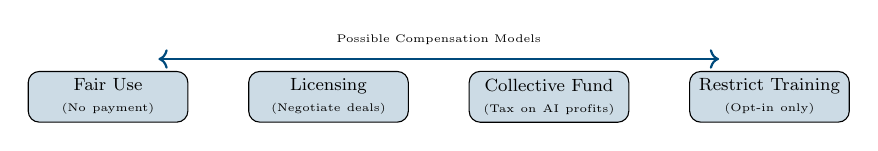
\begin{tikzpicture}[scale=0.8, transform shape]
        \node[draw, rounded corners, fill=primaryblue!20, text width=2.3cm, align=center, font=\footnotesize] at (0,0) (fair) {Fair Use\\{\tiny (No payment)}};
        \node[draw, rounded corners, fill=primaryblue!20, text width=2.3cm, align=center, font=\footnotesize] at (3.5,0) (license) {Licensing\\{\tiny (Negotiate deals)}};
        \node[draw, rounded corners, fill=primaryblue!20, text width=2.3cm, align=center, font=\footnotesize] at (7,0) (collect) {Collective Fund\\{\tiny (Tax on AI profits)}};
        \node[draw, rounded corners, fill=primaryblue!20, text width=2.3cm, align=center, font=\footnotesize] at (10.5,0) (ban) {Restrict Training\\{\tiny (Opt-in only)}};
        
        \draw[<->, thick, primaryblue] (0.8,0.6) -- (9.7,0.6);
        \node[above, font=\tiny] at (5.25,0.7) {Possible Compensation Models};
    \end{tikzpicture}
\end{frame}

%------------------------------------------------------
% SLIDE 48: Conclusion: Intellectual Property in the Digital Age
%------------------------------------------------------
\begin{frame}{Conclusion: Intellectual Property in the Digital Age}
    \begin{itemize}
        \item Intellectual property law developed for a physical world where copying was expensive and slow; digital technology has made copying instant, perfect, and nearly free---challenging every assumption.
        \item The central tension remains: \textbf{creators deserve recognition and reward} for their work, but \textbf{society benefits when knowledge flows freely}---every IP system must balance these values.
        \item New questions keep emerging: Who owns AI-generated content? Should you be able to repair your own tractor? Is training on copyrighted data fair use? How do we preserve digital culture?
        \item There are no perfect answers---IP involves genuine tradeoffs between competing goods, and different societies will continue to strike different balances.
    \end{itemize}
    
    \vspace{0.3em}
    
    \begin{block}{Key Takeaways}
        \small
        \textbf{1.} IP creates artificial scarcity to incentivize creation---but too much restriction harms innovation and access. \textbf{2.} Digital technology has disrupted every form of IP. \textbf{3.} The AI training debate may reshape copyright law for a generation. \textbf{4.} Your choices---what you create, share, and consume---shape this ongoing negotiation.
    \end{block}
\end{frame}

\end{document}